\chapter{Metoder}\label{ch:met}
I dette kapitel vil vi redegøre for hvilke UX metoder vi har valgt at bruge i vores evaluering af CodeAcademy. Vi har valgt at begge metoder skal være meget forskellige fra hinanden, så de kan give os forskellige perspektiver. Begge er funde igennem \textit{All About UX}\cite{AllAboutUX}.


\section{Affect Grid}\label{sec:AG}
Vi vil gerne vide, hvordan brugeres oplevelse ændrer sig under interaktion med Code Academy. Vi har altså brug for en metode, der kan anvendes til at indsamle data flere gange under vores evaluering. 

Under evaluering kan det dog være svært løbende at sætte sig ind i en bruger føler. Hvis evaluatoren hele tiden stiller dybdegående spørgsmål under evalueringen, risikerer vi at brugeren bliver trukket ud af interaktionen. Dette kommer til at have indflydelse på brugerens oplevelse af produktet. Det vil altså være bedst hvis brugen selv kunne angive hvordan de føler løbende under evalueringen. Helst uden at de skal tænke for meget over det. 

Metoden vi vælger at anvende hedder Affect Grid. Den er udviklet inden for psykologien af James A. Russel samt Anna Weiss og Gerald A. Mendelsohn \cite{AffectGrid}. Her angiver brugeren selv deres følelsesmæssige tilstand, også kendt som \textit{affect}, på det såkaldte Affect Grid. Et blankt affect grid kan ses på \cref{fig:affectgrid}. Grid'et har en størrelse på 9*9 felter, X-aksen angiver fornøjelse(pleasure) og Y-aksen angiver ophidselse(arousal). Et 1 på X-aksen betyder stærk misfornøjelse, mens et 9 betyder stærk fornøjelse. Ligeledes betyder 1 på Y-aksen stærk søvnighed og 9 betyder stærk ophidelse. Hele metoden baserer sig på, at fornøjelse og ophidelse er uafhængige  fra hinanden. 

\begin{figure}[h]
\centering
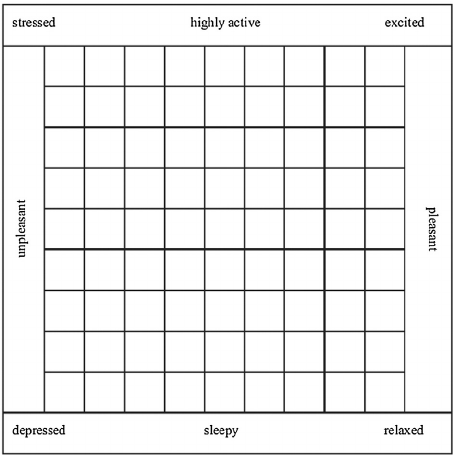
\includegraphics[width=0.6\textwidth]{affectgridbase.png}
\caption{Blank Affect Grid}
\label{fig:affectgrid}
\end{figure}

Ved anvendelse af dette grid kan en bruger nemt angive \textit{affect} ved at overveje deres nuværende fornøjelses- og ophidelsesniveau og derefter markere på gridet. Da dette ikke kræver meget af brugeren, regner vi med at der kan markeres flere gange under evalueringen, uden at brugeren trækkes ud af interaktionen. Derfor anvender vi Affect Grid til løbende at indsamle data om brugeres \textit{affect} under evalueringen.


\section{3E}\label{sec:3E}
Da vi også vil gerne indsamle noget mere kvalitativt om brugerens følelser for systemet. Det kan dog være svært at indsamle kvalitativ data løbende under selve forsøgs processen, da det typisk tager længere tid at for en brugere at give os den kvalitative data. Dette kan medføre at brugeren bliver revet ud af sin oplevelse af systemet, og evt. kan have det svært med at komme tilbage, da han da skal interegere med en testudøver som indsamler data, og ikke systemet.

Vi har derfor valgt at søge efter en metode som kan bruges på et episode plan, dvs. efter at en forsøgs person har interegeret med systemet, og som kan fange personens oplevelse af systemet. Til dette valgte vi at bruge metoden \textit{Expressing Experiences and Emotions} (\textit{3E}), som tillader en bruger nemt og på en useriøs måde at projektere sine følelser ned på en tegning, samtidigt med at han verbalt kan beskriver sine tanker bag systemet. Inden en forsøgs person begynder vil der allerede være tegnet en tændstiksmand, en talebobel og en tænkebobel på tegningen. Disse er med til at hjælpe en bruger til at projektere sine følelser, da de evt. kunne give tændstiksmanden et ansigt der viser deres følelser, eller de kunne tegne deres tanker om systemet i tankeboblen.

Et problem med \textit{3E} kan dog være at det kan være meget svært at analysere dataen bagefter. Da den data vi har indsamledt er meget subjektiv og kræver at vi foltolker folks tegninger. Det er mening at det at man beder brugeren om at beskrive sin tegning enten efter eller imens han tegner skal minimere denne fortolkning.


